\chapter{Real-Hardware Bridge Architecture}
\label{ch:hardware-bridge}

This chapter presents the architecture built to connect the
simulation-validated navigation stack of Chapter~\ref{ch:sim-stack}
to the physical QCar. Section~\ref{sec:rmw-incompatibility}
establishes why native ROS~2 communication with the robot's onboard
compute is not available, which motivates the TCP/JSON bridge
architecture of Section~\ref{sec:bridge-architecture}. The remaining
sections document the sensor and actuator correctness issues found
while bringing that bridge up to the same fidelity as the simulation
stack: LiDAR angle convention (Section~\ref{sec:lidar-angle}),
odometry (Section~\ref{sec:onboard-bridge-odom}), steering trim
(Section~\ref{sec:steering-trim}) and inter-machine clock
synchronisation (Section~\ref{sec:clock-offset}).

\section{Why Native ROS~2 Communication With the QCar Is Not Available}
\label{sec:rmw-incompatibility}

Two separate constraints rule out installing ROS~2 Humble directly
on the QCar's own compute. Either one alone would have forced the
bridge architecture of Section~\ref{sec:bridge-architecture}.
Together, they leave no realistic native alternative.

\paragraph{Storage.}
As described in Section~\ref{sec:qcar-platform}, the Jetson TX2's
32\,GB eMMC \cite{quanser2023qcar} already carries Ubuntu 18.04, ROS~1 Melodic, ROS~2
Dashing and Quanser's own HAL/PAL software. A second, full ROS~2
Humble installation needs its own client libraries, its own DDS
implementation and driver code to bridge ROS~2 to the HAL/PAL
layer. Fitting all of that into what remained of the 32\,GB was
judged unlikely, based on the typical size of a ROS~2 Humble
install. This constraint does not depend on whether Dashing and
Humble can otherwise talk to each other. Fixing DDS compatibility
would not, by itself, free up disk space.

\paragraph{The ROS~2 Dashing / Humble DDS Incompatibility.}
Independently of storage, this incompatibility was tested directly
rather than assumed. The QCar's onboard Jetson TX2 ships with ROS~2
Dashing (released 2019) pre-installed, while this project's
navigation stack targets ROS~2 Humble (released 2022). Section~\ref{sec:ros2-model}
established that ROS~2 nodes communicate via DDS participants that
must share a compatible discovery and wire protocol to find each
other at all. The working hypothesis at the start of this thesis's
hardware phase was that this would be a soft compatibility problem:
degraded performance, perhaps, but not a hard failure.

A minimal ROS~2 publisher (\texttt{demo\_nodes\_cpp talker}) on the
QCar and a minimal subscriber (\texttt{demo\_nodes\_py listener}) on
the development PC, both configured with the same
\texttt{ROS\_DOMAIN\_ID}, never established communication across
three repeated attempts. The talker was independently confirmed to
be actively publishing each time. The network layer itself was
systematically ruled out before concluding this was a
middleware-level problem. Raw UDP unicast passed cleanly in both
directions, including on the exact Fast~DDS discovery port for the
domain in use. No firewall was active on either host. An
explicit unicast-peers Fast~DDS XML profile, which bypasses
multicast-based discovery entirely, still failed to achieve
discovery. This isolates the failure to the DDS protocol
implementation itself: a genuine Fast~DDS protocol-version
incompatibility between the versions bundled with ROS~2 Dashing and
ROS~2 Humble respectively. Each RTPS message identifies the protocol
version its sender implements \cite{omg2014rtps}. Two peers
implementing different versions can fail to complete discovery even
when the underlying network path is sound. This is not a network,
firewall, or configuration problem that could be worked around
within ROS~2 itself.

This result rules out one further option that the storage constraint
alone would not: running a Humble-compatible container on the QCar
instead of a second native install. A Humble Docker container was
considered early on. It only partially sidesteps the storage
question: a container image adds its own storage overhead rather
than removing it. Nor does it address the protocol-version
incompatibility at the DDS transport layer at all.
The Dashing side of the link is fixed by what physically runs on the
vehicle's ROS~2 partition and cannot itself be upgraded without
departing from the vendor-supported software image.

\section{Bridge Architecture Overview}
\label{sec:bridge-architecture}

\begin{figure}[htbp]
  \centering
  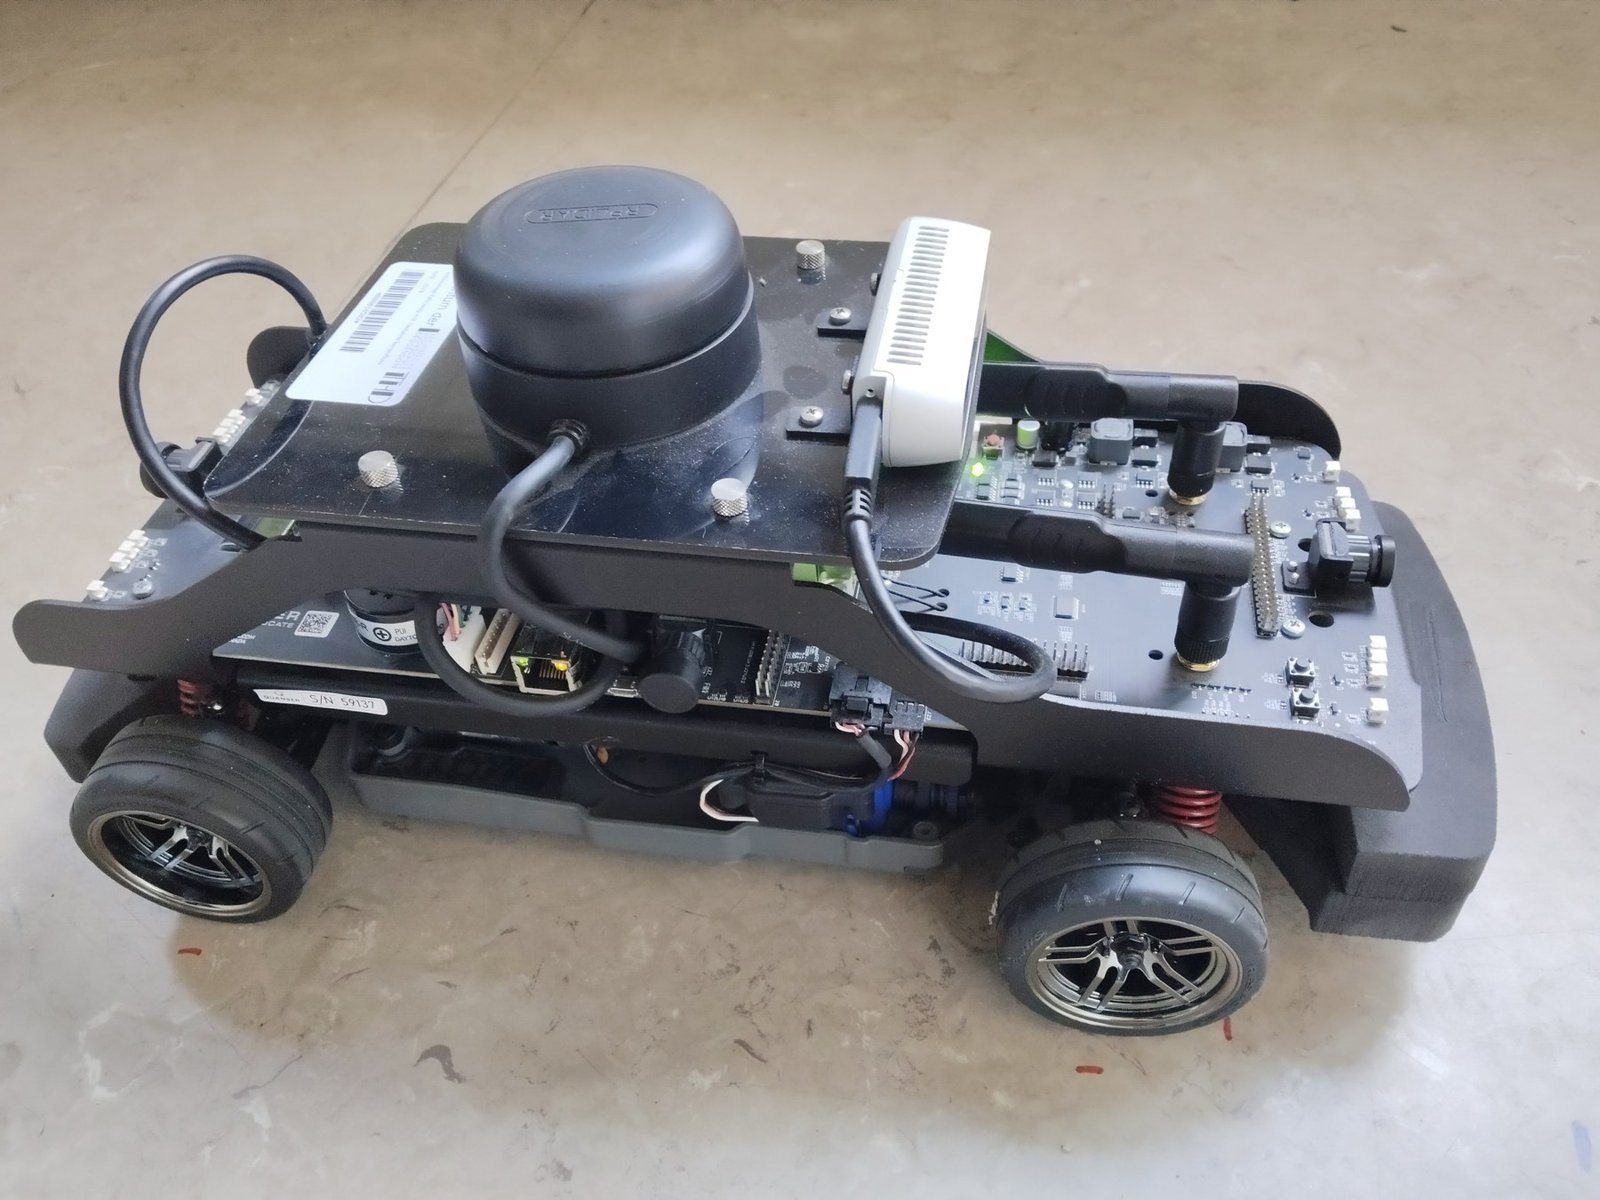
\includegraphics[width=0.75\textwidth]{figures/qcar-compute-sideview-photo.jpg}
  \caption[Side view of the QCar's onboard compute stack]{A side view of the physical QCar showing the onboard
    compute and sensing stack that this bridge architecture runs on:
    the RPLiDAR unit, the Jetson TX2 carrier board (with its wireless
    antennas and USB peripherals) and the wireless router used for
    the development PC's network link, all mounted above the chassis
    and drivetrain.}
  \label{fig:qcar-compute-sideview-photo}
\end{figure}

The architecture built in response uses no ROS~2 at all on the
QCar's own compute. Two plain Python processes run directly on the
Jetson TX2 (no \texttt{colcon} build, invoked as
\texttt{python3 <script>.py}):

\begin{itemize}
  \item \texttt{qcar\_bridge.py} -- a TCP server (port 5555) wrapping
    the Quanser HAL/PAL \texttt{QCar} object (Section~\ref{sec:qcar-platform}):
    receives newline-delimited JSON drive/steering commands and
    responds with odometry JSON over the same full-duplex connection.
  \item \texttt{qcar\_lidar\_node.py} -- a second TCP server (port
    5556) wrapping the LiDAR driver, streaming scan data as
    newline-delimited JSON.
\end{itemize}

On the development PC, a single node, \texttt{qcar\_relay\_node.py},
is the sole point of contact between ROS~2 and this TCP/JSON
protocol. It subscribes to \texttt{/cmd\_vel} and forwards commands
into the motor socket. The same node also publishes \texttt{sensor\_msgs/LaserScan}
on \texttt{/scan} and \texttt{nav\_msgs/Odometry} plus the
\texttt{odom} $\rightarrow$ \texttt{base} TF on \texttt{/odom}, from
data received back over both sockets. Every other node in the
navigation stack -- Nav2, AMCL, Cartographer, RViz -- interacts with
this relay node exactly as it would with the simulation's own drive
plugin. This requires no awareness that the underlying vehicle is real
hardware reached over a bespoke protocol rather than a co-located
Gazebo simulation.

Listing~\ref{lst:bridge-recv-loop} shows the command-receiving side of
this protocol inside \texttt{qcar\_bridge.py}'s main loop: incoming
TCP bytes are accumulated into a buffer and split on newlines. Each
complete line is then parsed as one JSON object, while a malformed
line is logged and discarded rather than allowed to crash the control loop.
This is deliberately fail-soft, since this loop is also driving the
physical motor and must keep running even if one message is corrupt.

\begin{lstlisting}[language=Python,caption={Newline-delimited JSON command parsing inside \texttt{qcar\_bridge.py}'s main loop.},label={lst:bridge-recv-loop}]
chunk = conn.recv(4096)
if chunk == b'':
    print('dev PC relay disconnected')
    break
buf += chunk
while b'\n' in buf:
    line, buf = buf.split(b'\n', 1)
    if not line.strip():
        continue
    try:
        cmd = json.loads(line)
        target_linear = float(cmd['linear_x'])
        angular_z = float(cmd['angular_z'])
        target_steering = compute_steering(target_linear, angular_z)
        last_cmd_time = time.time()
    except (ValueError, KeyError, TypeError):
        print('bad command line, ignoring:', line)
\end{lstlisting}

\paragraph{Why TCP, why newline-delimited JSON and why one socket per direction.}
Three protocol design choices underlie Listing~\ref{lst:bridge-recv-loop}
and are worth making explicit, since each addresses a specific
failure mode rather than being an arbitrary convenience. \textbf{TCP rather than UDP}: TCP guarantees in-order, complete
delivery of every byte sent (retransmitting silently on packet loss)
at the cost of unbounded, variable latency under loss, whereas UDP
offers low, predictable latency but silently drops or reorders
packets under loss with no delivery guarantee at all
\cite{rfc793tcp,rfc768udp}. For velocity
and steering commands, a stale duplicate or a dropped byte silently
corrupting the JSON stream is a worse failure than an occasional
extra tens of milliseconds of latency -- latency that the
\texttt{CMD\_TIMEOUT} watchdog in Section~\ref{sec:onboard-bridge-odom}
already treats as a safety condition regardless of its cause. TCP's
reliability guarantee won out over UDP's
lower-latency-but-lossy profile.

\textbf{Newline-delimited JSON rather than a fixed-length or
length-prefixed binary framing}: TCP is a byte stream with no
built-in concept of message boundaries, so \emph{some} framing scheme
is unavoidable. A length-prefixed binary format would be marginally
more compact, but a plain ASCII delimiter is trivially inspectable
with a bare \texttt{nc}/\texttt{telnet} session during debugging.
This was a real, exercised advantage throughout this project's
development, not a theoretical one. A plain delimiter also requires
no shared binary schema to keep in sync between the QCar-side Python
and dev-PC-side Python.

This is also why \texttt{buf} accumulates across \texttt{recv()}
calls, rather than assuming one \texttt{recv()} returns exactly one
message. TCP's byte-stream semantics make no guarantee that message
boundaries align with any particular \texttt{recv()} call's return:
a message can legitimately arrive split across two calls, or two
messages can arrive concatenated in one call.
Listing~\ref{lst:bridge-recv-loop}'s \texttt{while b'\textbackslash n' in buf}
loop handles both cases uniformly, by always operating on whatever
has accumulated so far.

\textbf{One full-duplex socket carrying both directions},
rather than two separate one-way sockets for commands and odometry:
a single TCP connection is inherently bidirectional, since each
endpoint can read and write independently on the same socket.
Section~\ref{sec:onboard-bridge-odom}'s later addition of odometry
sent back to the relay required no new listening port or
connection -- only using a direction of the existing socket that
had, until then, been opened but left unread.

Figure~\ref{fig:bridge-architecture} shows the complete command and
sensor data path across both machines and both TCP sockets, matching
exactly the components and topics named above.

\begin{figure}[htbp]
  \centering
  \resizebox{\textwidth}{!}{%
  \begin{tikzpicture}[
      node distance=8mm and 14mm,
      box/.style={draw, rounded corners, align=center, minimum height=9mm,
        minimum width=32mm, font=\small},
      hostbox/.style={draw, dashed, inner sep=6mm, rounded corners},
      lbl/.style={font=\scriptsize, align=center},
      arr/.style={-{Latex[length=2mm]}, thick}
    ]

    % --- Development PC (ROS 2 Humble side) ---
    \node[box] (nav2) {Nav2 / AMCL /\\Cartographer};
    \node[box, below=of nav2] (relay) {\texttt{qcar\_relay\_node.py}};
    \node[lbl, left=2mm of relay, align=right, text width=18mm]
      {publishes\\\texttt{/scan}, \texttt{/odom}\\subscribes\\\texttt{/cmd\_vel}};

    \node[hostbox, fit=(nav2)(relay), label={[font=\small\bfseries]above:Development PC (ROS~2 Humble)}] (pcbox) {};

    % --- QCar Jetson TX2 (no ROS 2) ---
    \node[box, right=48mm of nav2] (bridge) {\texttt{qcar\_bridge.py}\\(TCP :5555)};
    \node[box, below=of bridge] (lidarnode) {\texttt{qcar\_lidar\_node.py}\\(TCP :5556)};
    \node[box, right=of bridge, yshift=-4mm] (hal) {Quanser HAL/PAL\\\texttt{QCar} object};
    \node[box, below=of hal] (motor) {Motor, servo,\\encoders, LiDAR};

    \node[hostbox, fit=(bridge)(lidarnode)(hal)(motor), label={[font=\small\bfseries]above:QCar Jetson TX2 (no ROS~2)}] (qcarbox) {};

    % --- Vertical flow inside each host ---
    \draw[arr] (nav2) -- (relay);
    \draw[arr] (bridge) -- (hal);
    \draw[arr] (lidarnode.east) -- (hal.west |- lidarnode.east);
    \draw[arr] (hal) -- (motor);

    % --- Cross-machine TCP/JSON links ---
    \draw[arr] (relay.north east) to[bend left=12]
      node[lbl, above, sloped]{JSON drive/steer cmd}
      (bridge.south west);
    \draw[arr] (bridge.south west) to[bend left=12]
      node[lbl, below, sloped]{JSON odometry}
      (relay.north east);
    \draw[arr] (lidarnode.west) to[bend right=8]
      node[lbl, below, sloped]{JSON scan}
      (relay.south east);

  \end{tikzpicture}%
  }
  \caption[Command/sensor data path: Nav2 to physical actuators]{Command and sensor data path from the Nav2 stack to the
    physical actuators and back. Both cross-machine links are
    newline-delimited JSON over TCP (ports 5555 and 5556); no ROS~2
    process runs on the QCar's own compute at any point in this
    path.}
  \label{fig:bridge-architecture}
\end{figure}

Both onboard TCP servers were built to handle \texttt{SIGTERM}
identically to \texttt{SIGINT} -- a deliberate correctness fix, not
a default. Python does not automatically translate a plain
\texttt{pkill}'s default \texttt{SIGTERM} into a caught, clean-exit
signal the way it does for \texttt{SIGINT} (Ctrl-C). An earlier
plain \texttt{pkill} against the LiDAR process left the physical
LiDAR unit spinning after the owning process had already exited --
both a battery drain and a safety concern for anyone near the
vehicle. Section~\ref{sec:safe-shutdown} presents the resulting
documented shutdown procedure in full.

\section{LiDAR Angle-Convention Correction}
\label{sec:lidar-angle}

The first sensor-correctness issue found while bringing up
visualisation of the bridged data (\texttt{robot\_state\_publisher} +
\texttt{joint\_state\_publisher} + RViz, no Gazebo) was a LiDAR
angle-binning defect in \texttt{qcar\_lidar\_node.py}: obstacles
rendered in RViz did not appear at their true bearing relative to the
rendered robot model. This required \emph{two} stacked, independent
corrections, not one -- a clockwise-to-counter-clockwise direction
flip \emph{and} a $+\ang{90}$ rotational offset between the LiDAR's
zero-reference bearing and the vehicle's own forward direction. The
first attempted fix (direction only) produced a result that was
itself the tell that a second error remained. It exactly mirrored
the original error about the vehicle's forward axis, rather than
correcting it -- the expected signature of fixing only a sign error
while a separate rotational offset error is still present. The
final, verified-correct transform is

\begin{equation}
  \theta_{\text{target}} = \operatorname{wrap}_{(-\pi,\,\pi]}\!\left(-\theta_{\text{lidar}} + \frac{\pi}{2}\right), \label{eq:lidar-angle-fix}
\end{equation}

This transform was verified against a real obstacle at a known
bearing (the vehicle's physical right side). The check used the
rendered robot model's own orientation in RViz, not the screen's raw
left/right, since screen left/right depends on the RViz camera's own
facing direction and is not a reliable reference on its own.

Listing~\ref{lst:lidar-angle-code} shows Equation~\ref{eq:lidar-angle-fix}
as implemented in \texttt{qcar\_lidar\_node.py}: each raw
\texttt{(angle, distance)} sample from the HAL is transformed, wrapped
into $(-\pi,\pi]$ via \texttt{atan2} and binned onto the fixed
360-sample grid a ROS~2 \texttt{LaserScan} message requires. The HAL
does not guarantee its raw samples already arrive pre-gridded in
order, so this binning step is necessary independently of the angle
correction itself.

\begin{lstlisting}[language=Python,caption={LiDAR angle correction and grid binning (\texttt{qcar\_lidar\_node.py}).},label={lst:lidar-angle-code}]
increment = (2.0 * math.pi) / NUM_MEASUREMENTS
ranges = [float('inf')] * NUM_MEASUREMENTS
for angle, dist in zip(lidar.angles, lidar.distances):
    target = -angle + math.pi / 2
    normalized = math.atan2(math.sin(target), math.cos(target))
    idx = int(round((normalized + math.pi) / increment)) % NUM_MEASUREMENTS
    if RANGE_MIN <= dist <= RANGE_MAX:
        ranges[idx] = float(dist)
\end{lstlisting}

\paragraph{Worked example: why a direction flip alone is not enough.}
Equation~\ref{eq:lidar-angle-fix}'s two-part correction is easiest to
see by tracing a few canonical raw LiDAR angles
$\theta_{\text{lidar}}$ through the transform
$\theta_{\text{target}} = \operatorname{wrap}(-\theta_{\text{lidar}} + \pi/2)$
in Table~\ref{tab:lidar-worked-example}. A \emph{direction-flip-only}
correction ($\theta_{\text{target}} = -\theta_{\text{lidar}}$, no
$+\pi/2$ term) would map the same four raw angles to
$0, -\pi/2, \pi, \pi/2$ respectively -- every value rotated exactly
\ang{90} short of the fully corrected column. This is precisely the
signature Section~\ref{sec:lidar-angle} describes: a direction-only
fix mirrors the error about the vehicle's forward axis rather than
removing it. Negating the angle alone corrects the sense of
increasing angle (clockwise vs.\ counter-clockwise), without also
correcting \emph{where zero itself points} -- two logically
independent properties of an angular convention. This is exactly why
this bug needed two independent corrections, not one.

\begin{table}[htbp]
  \centering
  \caption{Illustrative raw-to-corrected LiDAR angle mapping (Equation~\ref{eq:lidar-angle-fix}).}
  \label{tab:lidar-worked-example}
  \begin{tabular}{@{}lcccc@{}}
    \toprule
    $\theta_{\text{lidar}}$ (raw) & $0$ & $\pi/2$ & $\pi$ & $-\pi/2$ \\
    \midrule
    $\theta_{\text{target}}$ (corrected) & $\pi/2$ & $0$ & $-\pi/2$ & $\pi$ \\
    \bottomrule
  \end{tabular}
\end{table}

\section{Wheel Odometry over the Bridge}
\label{sec:onboard-bridge-odom}

Mapping (Cartographer, Section~\ref{sec:cartographer}) was
successfully brought up on real hardware using scan-matching alone,
with \texttt{use\_odometry: false} / \texttt{provide\_odom\_frame:
true} in the Cartographer configuration -- meaning the initial bridge
implementation required no odometry extension at all for mapping to
work end-to-end. Localisation (AMCL) does not share this property. Unlike
Cartographer's self-contained scan matching, AMCL looks up a
live \texttt{odom} $\rightarrow$ \texttt{base} TF at every scan
callback as its motion-model input. As a result, the wheel-odometry
extension originally scoped only for the mapping phase became a hard
requirement once navigation (Nav2/AMCL) was brought up.

\texttt{qcar\_bridge.py} was extended with an \texttt{Odometry} class
implementing the same bicycle-model dead-reckoning integration as
Equations~\ref{eq:bicycle-x}--\ref{eq:bicycle-theta}. The resulting
odometry is sent back to the relay over the same already-full-duplex
TCP connection the drive commands arrive on; the reverse direction of
this connection had previously been opened but its data discarded.
\texttt{qcar\_relay\_node.py} parses this stream and publishes both
\texttt{/odom} and the corresponding TF. Tested in isolation before
layering Nav2 on top, the resulting odometry published at
approximately 45\,Hz. A 3-second commanded straight-line drive at
\SI{0.3}{\meter\per\second} produced $x \approx \SI{1.25}{\meter}$,
$v \approx \SI{0.37}{\meter\per\second}$, $y \approx 0$ -- consistent
with straight-line motion at close to the commanded speed. This
confirmed the odometry was working before the full navigation stack
was brought up on top of it.

Listing~\ref{lst:odometry-class} shows the \texttt{Odometry} class in
full. \texttt{update()} is called once per control-loop cycle with
the raw encoder count and the current commanded steering angle and
directly implements the bicycle-model relationship of
Equations~\ref{eq:bicycle-x}--\ref{eq:bicycle-theta}. Encoder-count
deltas become a travelled distance via the fixed
\texttt{METERS\_PER\_COUNT} conversion, from which velocity and yaw
rate follow; $x$, $y$ and yaw are then integrated forward exactly as
in the continuous-time model.

\begin{lstlisting}[language=Python,caption={Bicycle-model dead-reckoning odometry (\texttt{qcar\_bridge.py}).},label={lst:odometry-class}]
class Odometry:
    def __init__(self):
        self.x = 0.0
        self.y = 0.0
        self.yaw = 0.0
        self.last_encoder = None

    def update(self, encoder_counts, steering, dt):
        if self.last_encoder is None:
            self.last_encoder = encoder_counts
        delta_counts = encoder_counts - self.last_encoder
        self.last_encoder = encoder_counts

        distance = delta_counts * METERS_PER_COUNT
        v = distance / dt
        yaw_rate = v * math.tan(steering) / WHEELBASE

        self.yaw += yaw_rate * dt
        self.x += distance * math.cos(self.yaw)
        self.y += distance * math.sin(self.yaw)

        return {'x': self.x, 'y': self.y, 'yaw': self.yaw,
                'v': v, 'yaw_rate': yaw_rate}
\end{lstlisting}

\paragraph{From raw encoder counts to metres.}
\texttt{METERS\_PER\_COUNT} (documented in \texttt{qcar\_bridge.py} as
$\frac{0.01977}{2880}$) is itself a small derived constant, not a
directly measured one. 2880 is the number of raw encoder counts per
one full revolution of the motor shaft, as documented in the Quanser
HAL manual \cite{quanser2023qcar} for this drive motor/encoder
pairing. \SI{0.01977}{\meter} is the linear distance one rear-wheel
revolution advances the vehicle -- the wheel's rolling circumference,
folding in the fixed gear ratio between motor shaft and wheel. Their
ratio converts a raw encoder delta directly into a travelled distance
in one multiplication, with no separate gear-ratio or
wheel-circumference term needed at the call site.

\paragraph{The integration is forward Euler, not an exact arc.}
Line-by-line, \texttt{update()} performs a standard forward-Euler
discretisation of Equations~\ref{eq:bicycle-x}--\ref{eq:bicycle-theta}.
It advances \texttt{self.yaw} by \texttt{yaw\_rate * dt} \emph{first},
then immediately uses that already-updated yaw to project the
travelled \texttt{distance} onto $x$ and $y$ via
$\cos(\text{yaw})$/$\sin(\text{yaw})$. This effectively assumes the
vehicle's heading was already at its new value for the entirety of
this cycle's straight-line displacement, rather than integrating the
true curved arc the vehicle followed while turning during the
interval.

This is a standard, deliberate simplification, matching how
Chapter~\ref{ch:sim-stack}'s simulation-side plugin also integrates
its own motion incrementally rather than analytically per step. Its
error shrinks toward zero as the control loop's period \texttt{dt}
shrinks, but it is not exact for any nonzero \texttt{yaw\_rate * dt}.
At this project's \SI{50}{\hertz} control rate
(Section~\ref{sec:bridge-architecture}), \texttt{dt} is small enough
that the resulting error is negligible next to this thesis's other,
much larger sources of odometry inaccuracy, such as steering trim
and throttle calibration. It is still worth naming explicitly as a
non-zero, if small, contributor to dead-reckoning drift over a long
enough drive.

\section{Steering-Trim Calibration}
\label{sec:steering-trim}

A small but consistent steering bias was present on this specific
chassis: the vehicle drifted laterally under a nominally straight,
zero-steering command. The physical steering linkage
could not be adjusted to correct it mechanically. The fix was
implemented in software instead, as a constant offset
(\texttt{STEERING\_TRIM}, an early estimate of \SI{-0.08}{\radian},
later refined to \SI{-0.087}{\radian} in
Section~\ref{sec:steering-gain} below) applied only at the point the
steering command is written to the servo. Calibration proceeded in
two stages: an initial static test (motor off, holding candidate
angles and judging visually against a reference, preserved as
\texttt{calibrate\_steering.py} for future re-calibration) narrowed
the value to roughly the right range. A series of real
straight-line driving tests (drive a known distance, measure the
resulting lateral offset, compute
$\delta_{\text{trim}} = \arctan(\text{offset}/\text{distance})$)
refined it further. This data carried real measurement noise. Lateral offset depends on
the vehicle's initial aim at the start of each test run, not purely
on trim, so the calibration deliberately did not over-fit a precise
value from only two data points. A
consistent directional nudge toward zero observed drift converged
faster in practice than attempting a precise interpolation.

This first-pass value was accepted once a \SI{4.4}{\meter} test drive
showed no reported drift. It is described as ``almost accurate,'' a
deliberate acceptance of a small residual rather than a claim of
exact zero. As the next section shows, it was in fact only half of
the real correction this vehicle needed.

\subsection{Steering Gain as a Second, Independent Nonlinearity}
\label{sec:steering-gain}

The trim calibration above corrects only the steering command's
\emph{offset} -- what the vehicle does at a commanded angle of zero.
It says nothing about whether a nonzero commanded angle produces the
correct amount of real wheel deflection. For a long period of
this project nobody had verified that separately. The gap surfaced
directly during Nav2 integration (Chapter~\ref{ch:nav-integration}):
I reported that autonomous navigation on real
hardware was ``not turning as well as sim,'' a complaint that a pure
offset error cannot explain, since an offset only shifts the
zero-point and leaves proportionality untouched.

\paragraph{Steering-gain test.} With a fresh battery fitted and
the test speed raised to \SI{0.4}{\meter\per\second}, confirmed via
logged velocity to sit safely above the stiction floor, a seven-point
sweep of commanded steering angles was driven, each a fresh
\SI{1}{\meter} arc from a consistent physical start pose.
\texttt{STEERING\_TRIM} was held at zero throughout, so the commanded
value was exactly what reached \texttt{car.write()}. The real wheel angle implied by
each measured lateral deviation was back-solved from the same
circular-arc geometry as the trim calibration above
($R = L/\tan\delta$, $y = R(1-\cos(s/R))$, wheelbase
$L=\SI{0.25725}{\meter}$), using bisection rather than a closed-form
inverse since the forward relationship is transcendental in $\delta$.
Table~\ref{tab:steering-gain-sweep} presents the results.

\begin{table}[htbp]
  \centering
  \caption{Commanded steering angle versus implied real wheel angle (\texttt{STEERING\_TRIM}=0).}
  \label{tab:steering-gain-sweep}
  \begin{tabular}{@{}cc@{}}
    \toprule
    Commanded angle (rad) & Implied real angle (rad) \\
    \midrule
    $0.00$ & $+0.112$ \\
    $-0.05$ & $+0.052$ \\
    $-0.08$ & $+0.018$ \\
    $-0.085$ & $+0.005$ \\
    $-0.09$ & $0.000$ \\
    $-0.10$ & $-0.021$ \\
    $-0.12$ & $-0.062$ \\
    \bottomrule
  \end{tabular}
\end{table}

\begin{figure}[htbp]
  \centering
  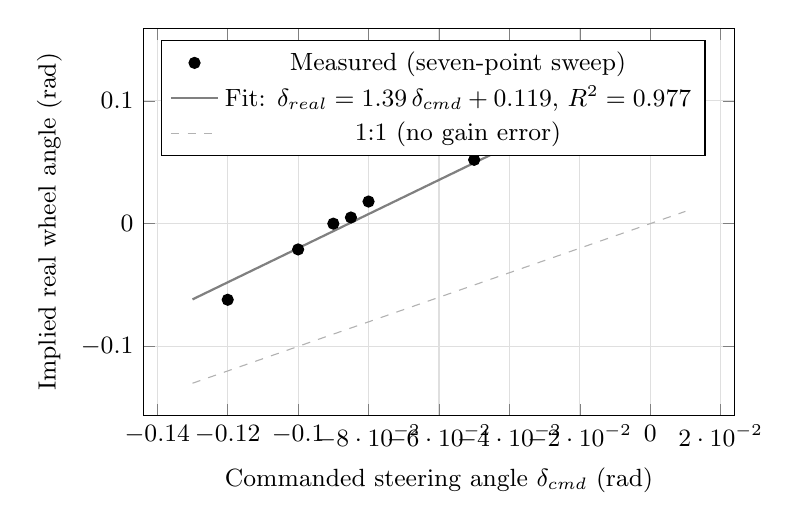
\begin{tikzpicture}
    \begin{axis}[
        width=0.75\textwidth, height=6.5cm,
        xlabel={Commanded steering angle $\delta_{\text{cmd}}$ (rad)},
        ylabel={Implied real wheel angle (rad)},
        grid=major, grid style={gray!25},
        legend pos=north west, legend style={font=\small},
        label style={font=\small}, tick label style={font=\small}
      ]
      \addplot[only marks, mark=*, mark size=2pt, color=black]
        coordinates {(0.00,0.112) (-0.05,0.052) (-0.08,0.018)
          (-0.085,0.005) (-0.09,0.000) (-0.10,-0.021) (-0.12,-0.062)};
      \addlegendentry{Measured (seven-point sweep)}
      \addplot[domain=-0.13:0.01, samples=2, thick, color=gray]
        {1.39*x + 0.119};
      \addlegendentry{Fit: $\delta_{\text{real}}=1.39\,\delta_{\text{cmd}}+0.119$, $R^2=0.977$}
      \addplot[domain=-0.13:0.01, samples=2, dashed, color=gray!60]
        {1.00*x};
      \addlegendentry{1:1 (no gain error)}
    \end{axis}
  \end{tikzpicture}
  \caption[Commanded vs.\ implied real steering angle]{Commanded versus implied real steering angle
    (Table~\ref{tab:steering-gain-sweep}), with the fitted regression
    line against the 1:1 relationship a gain-free kinematic model
    would predict. The fitted slope of 1.39 is the multiplicative gain
    error itself; the vertical offset between the two lines at
    $\delta_{\text{cmd}}=0$ separately reflects the zero-point trim
    before it was corrected.}
  \label{fig:steering-gain-fit}
\end{figure}

The relationship is clean, monotonic and shows no sign flips or
stalls. A least-squares linear fit,
$\delta_{\text{real}} = m \, \delta_{\text{cmd}} + c$, gives
$m = 1.39$, $c = \SI{0.119}{\radian}$, $R^2 = 0.977$ (the two
largest-magnitude commands sit slightly above the fitted line, a mild
hint of additional curvature at large angles not investigated
further). Two conclusions follow directly. The true zero-point
trim is $\delta_{\text{cmd}} = -0.09$, not the $-0.08$ found by the
coarser static test above, pinned by direct interpolation between
the $-0.085$ (implied $+0.005$) and $-0.09$ (implied $0.000$) rows.
Independently of the trim value entirely, the real wheel
also turns approximately 39\% \emph{further} than the kinematic model's
commanded angle implies for any non-zero command. This is a genuine
multiplicative gain error, not an offset and one that a pure trim
correction cannot fix. This gain error is a strong candidate explanation for the
original complaint that motivated the investigation. Nav2's planner
and MPPI controller both assume the kinematic model of
Section~\ref{sec:true-ackermann} maps 1:1 onto real wheel angle. A
vehicle that over-rotates by 39\% for every commanded turn would
visibly overshoot turns and cut corners tighter than planned,
exactly the symptom reported.

\paragraph{Fix and validation.} A documentation check first confirmed
that no factory steering calibration exists to consult. The Quanser
hardware manual \cite{quanser2023qcar} documents only the raw servo
command range and the physical maximum wheel angle
(Table~\ref{tab:app-safety-limits}). The HAL's own
\texttt{steeringBias} construction parameter was confirmed left at
its default of zero in \texttt{qcar\_bridge.py} -- nothing at the
firmware level was fighting or duplicating the software correction.
\texttt{STEERING\_GAIN = 1.39} (Listing~\ref{lst:trim-split}'s
\texttt{apply\_trim()}, which pre-divides the kinematic angle by this
constant before adding \texttt{STEERING\_TRIM}) was set directly from
this regression. The trim itself was then refined further, from three
repeated trials each at commanded $-0.08$, $-0.085$ and $-0.09$ (to
average out human placement and measurement noise): the zero-crossing
of the three averaged measurements gave a final
\texttt{STEERING\_TRIM = -0.087}. A dedicated validation drive commanded a real kinematic turn of
\SI{0.15}{\radian} over a \SI{1}{\meter} arc at
\SI{0.4}{\meter\per\second}, predicting \SI{28.5}{\centi\meter} of
lateral deflection. The measured deflection was \SI{27}{\centi\meter},
a residual error of $\approx$5.6\%, down from $\approx$39\% with no
gain correction at all. The fix was subsequently
confirmed in genuine closed-loop use. After re-running autonomous
Nav2 navigation on the physical vehicle post-deployment, my
direct assessment was that turning behaviour had visibly
improved. This is consistent with the gain error having been the
dominant cause of the original complaint rather than merely a
contributing factor.

As with the throttle calibration constants of
Section~\ref{sec:final-calibration}, both \texttt{STEERING\_GAIN} and
\texttt{STEERING\_TRIM} are per-unit values, expected to differ on a
different physical chassis. The empirical sweep-and-regression
\emph{method} used to find them is the transferable result, not the
specific numbers. One operational caution from this investigation is
also worth recording: testing a previously untested steering-angle
magnitude can produce more real curvature than expected. Available
clearance should be confirmed in the new command's actual curve
direction before testing it, not only in directions already validated
at smaller magnitudes.

\subsection{A Trim-Placement Bug and the ``Apply at the Actuator Boundary'' Principle}
\label{sec:trim-boundary-principle}

The first implementation of this trim contained a real bug worth
recording as a general principle for any per-unit hardware
calibration constant, not only this one. It folded the trim into the
\emph{same} steering value used both for the real servo command
\emph{and} for the odometry dead-reckoning calculation in
Section~\ref{sec:onboard-bridge-odom}. The entire purpose of
the trim is to make the real wheels read approximately zero deflection
despite a nonzero servo command. Feeding that same trimmed value into
odometry made the dead-reckoning model believe the wheels were
deflected by the trim amount, even while the vehicle was in reality
driving dead straight. A live test briefly exposed this directly: a
straight-line drive of approximately \SI{2.8}{\meter} produced a
fictitious $y \approx \SI{-1.72}{\meter}$ in the odometry output, a
spurious $\sim$\ang{30} curve that did not correspond to any real
vehicle motion.

The fix separated \texttt{compute\_steering()} (returns the
untrimmed, kinematic steering angle, used for odometry) from a new
\texttt{apply\_trim()} (computes the real servo command, called only
immediately before the HAL write), shown together in
Listing~\ref{lst:trim-split}. \texttt{target\_steering} is
\texttt{compute\_steering()}'s untrimmed return value. It is also what
Listing~\ref{lst:odometry-class}'s \texttt{odom.update()} call is
given. \texttt{apply\_trim()} is invoked only once, at the
\texttt{car.write()} call site itself.

\begin{lstlisting}[language=Python,caption={The kinematic-steering / servo-trim split (\texttt{qcar\_bridge.py}).},label={lst:trim-split}]
def compute_steering(linear_x, angular_z):
    # Returns the KINEMATIC (untrimmed) angle - used for odometry.
    # STEERING_TRIM must NOT be folded in here (see prose above).
    if abs(linear_x) < 1e-2:
        steer = 0.0
    else:
        steer = math.atan(WHEELBASE * angular_z / linear_x)
    return max(-MAX_STEER_CMD, min(MAX_STEER_CMD, steer))


def apply_trim(kinematic_steering):
    # Converts a real/kinematic steering angle into the servo command
    # that achieves it on this vehicle - call only right before
    # car.write(), never upstream of odometry or anything else that
    # treats its input as the true physical wheel angle.
    return max(-MAX_STEER_CMD,
               min(MAX_STEER_CMD,
                   kinematic_steering / STEERING_GAIN + STEERING_TRIM))
\end{lstlisting}

Re-verified with the same drive
command, the odometry then correctly read $y \approx 0$. The general
principle this illustrates is stated here explicitly, because it is
expected to generalise to any future per-unit hardware calibration
constant on this or a similar platform: a calibration constant
compensating for a specific actuator's physical imperfection should
be applied \emph{as late as possible, immediately at the actuator
boundary}. It should never be applied upstream of any computation,
such as odometry, that treats its input as an accurate, ground-truth
kinematic quantity.

\section{Clock Synchronisation and the Receipt-vs-Capture Timestamp Bug}
\label{sec:clock-offset}

The first real navigation-goal test I ran, once mapping,
localisation and the fixes above were all in place, surfaced a new
symptom: sudden AMCL localisation jumps and visible path deviation
on both straight and curved segments. The description of what was actually observed was
distinctive: LiDAR scan shape stays internally coherent, but the
entire scan rigidly shifts and appears to track the robot's motion,
``like the skeleton of the map is moving.'' That, together with an
explicit instinct that this might be a transform-related issue
rather than a tuning problem, pointed toward a \emph{timing} rather
than a spatial or gain-tuning cause -- and this proved correct.

\texttt{/scan} (port 5556) and \texttt{/odom} (port 5555) are two
independent TCP streams, each subject to its own, uncorrelated
network jitter -- this link had already been measured showing
\SIrange{87}{300}{\milli\second} of variable latency.
\texttt{qcar\_relay\_node.py} had been stamping both incoming
streams with \texttt{self.get\_clock().now()} at the moment of TCP
\emph{receipt} on the development PC, rather than at the moment of
sensor \emph{capture} on the QCar. Because the two streams' receipt
times are decorrelated, a late-arriving scan could be paired against
an odometry sample purely by receipt-time coincidence. In real
physical time, that odometry sample could already be stale by a
different, independent amount. This produces exactly the observed symptom: a
LiDAR scan that is internally self-consistent but rigidly offset
relative to the map, tracking the robot's own recent motion.

The fix required both machines' clocks to be related, not merely
each stream's own internal timing corrected. A round-trip-corrected
NTP-style offset measurement (five clustered trials of
$\text{offset} = t_{\text{remote}} - (t_1+t_2)/2$ around an SSH
\texttt{date} call) found a genuine $\sim$\SI{0.50}{\second} clock
offset between the two machines -- a naive sequential comparison
without the round-trip correction would have overstated this by also
counting SSH connection-setup time as clock skew.

\paragraph{Why the round-trip correction is needed.}
A naive measurement works like this: record a local timestamp $t_1$,
SSH into the QCar and read its clock to get $t_{\text{remote}}$, then
compute $t_{\text{remote}} - t_1$. This conflates two effects that a
single one-way measurement cannot separate. One is the genuine clock offset
between the two machines. The other is the real, nonzero time the
SSH round trip itself takes to establish a connection and execute
the remote command, which inflates the apparent gap in one direction
only.

The correction used here follows the same symmetric-delay assumption
underlying NTP itself \cite{rfc5905ntp}: record a second local timestamp $t_2$
immediately after the remote reply arrives. Treat the remote
reading as having been taken at the network's best available
estimate of the corresponding local instant -- the midpoint
$(t_1+t_2)/2$. This assumes the outbound and return legs of the
round trip take approximately equal time, which is reasonable for a
short, otherwise idle local-network SSH round trip, but would not be
for a highly asymmetric link. Averaging five such trials, rather
than trusting a single one, further reduces the influence of any one
trial's round-trip time deviating unusually from that
symmetric-delay assumption.

This offset was deliberately \emph{not} corrected via a system-level
NTP/chrony configuration, since the QCar is shared laboratory
hardware. A persistent system configuration pointing it at one
researcher's personal development machine as a time reference is
not appropriate to leave on shared infrastructure. Instead,
\texttt{qcar\_bridge.py} and \texttt{qcar\_lidar\_node.py} were
changed to stamp every message with their own local
\texttt{time.time()} at the moment of capture, added as a
\texttt{'t'} field in the JSON payload. \texttt{qcar\_relay\_node.py}
gained a \texttt{qcar\_clock\_offset} parameter and a
\texttt{qcar\_time\_to\_stamp()} helper that converts a QCar-local
capture timestamp into its development-PC-clock equivalent, applied
consistently to both the \texttt{/odom}+TF and \texttt{/scan}
publication paths. Listing~\ref{lst:clock-offset-code} shows the
conversion.

\begin{lstlisting}[language=Python,caption={Converting a QCar-local capture timestamp to the development PC's clock (\texttt{qcar\_relay\_node.py}).},label={lst:clock-offset-code}]
def qcar_time_to_stamp(qcar_time, qcar_clock_offset):
    '''Converts a QCar-clock time.time() reading into a
    builtin_interfaces/Time on this machine's clock, correcting for
    the measured offset between the two machines' independent,
    unsynchronized clocks.'''
    corrected = qcar_time - qcar_clock_offset
    sec = int(corrected)
    nanosec = int(round((corrected - sec) * 1e9))
    return Time(sec=sec, nanosec=nanosec)
\end{lstlisting}

\begin{table}[htbp]
  \centering
  \caption{Diagnostic measurements underlying the clock-offset fix.}
  \label{tab:clock-offset}
  \begin{tabular}{@{}ll@{}}
    \toprule
    Quantity & Value \\
    \midrule
    Network latency (TCP link, both ports) & \SIrange{87}{300}{\milli\second} (variable) \\
    Measured clock offset (round-trip corrected, initial session) & $\approx \SI{0.50}{\second}$ \\
    Measured clock offset (persistent-connection method, final session) & $\approx \SI{0.019}{\second}$ \\
    \texttt{qcar\_clock\_offset} launch parameter (final verified session) & \texttt{0.019} \\
    \bottomrule
  \end{tabular}
\end{table}

\paragraph{A measurement artifact found in a later session.} A
subsequent hardware session revisited this offset and found the
round-trip correction above still carries a hidden bias when each of
the five trials opens its own fresh SSH connection. Repeating the
measurement that day gave a wide, noisy spread (mean
\SI{0.93}{\second}, range \SI{0.28}{\second}--\SI{1.58}{\second})
rather than a tight, repeatable figure. Clock drift accumulates
gradually and could not explain a spread this wide within one
sitting. The actual cause was SSH's own per-connection handshake:
opening a brand-new connection for every trial front-loads that
handshake delay onto the outbound leg only, which breaks the
equal-outbound/return-delay assumption the round-trip correction
itself depends on.

Re-measuring over a single, persistent SSH connection
(\texttt{ControlMaster} multiplexing, no fresh handshake per sample)
removed this asymmetry directly. The result converged tightly to
\SI{0.019}{\second} across eleven of twelve samples, roughly two
orders of magnitude smaller than the \SI{0.50}{\second} figure
originally measured. The diagnosis and fix earlier in this section
remain correct in substance: an uncorrected receipt-timestamp
mismatch of this kind genuinely produces the display artefact
described here. Only the specific magnitude measured at the time was
inflated by the fresh-connection method's own hidden asymmetry, not
by a flaw in the receipt-vs-capture diagnosis itself.
\texttt{qcar\_clock\_offset = 0.019} is the value used in this
project's final hardware configuration.

\section{Safe Shutdown Procedure}
\label{sec:safe-shutdown}

Because two of the four processes in this bridge run directly on
physical hardware with no supervising ROS~2 lifecycle to fall back
on, this project established and documented a fixed shutdown
sequence, using \texttt{SIGINT} exclusively rather than a plain
\texttt{pkill} (per the signal-handling fix in
Section~\ref{sec:bridge-architecture}):
(1)~stop \texttt{qcar\_relay\_node.py} on the development PC;
(2)~stop the visualisation launch process group (RViz may itself
segfault on exit, a known, harmless Qt/OpenGL quirk on this system --
worth confirming it has actually exited rather than assuming);
(3)~stop \texttt{qcar\_lidar\_node.py} on the QCar;
(4)~stop \texttt{qcar\_bridge.py} on the QCar (requires \texttt{sudo}).
This project's own operational experience found it is not sufficient
to trust that the sequence \emph{was run}. On one occasion, the
motor bridge was still listening on its TCP port after I
believed it had been stopped. The documented procedure therefore
explicitly includes confirming both TCP ports (5555, 5556) are
released on the QCar (\texttt{ss -tlnp}) before considering the
vehicle idle.

\section{Summary}
\label{sec:hardware-bridge-summary}

This chapter's bridge architecture makes the physical QCar appear,
from the perspective of every ROS~2 node in the navigation stack, as
an ordinary \texttt{/cmd\_vel}-in, \texttt{/odom}/\texttt{/scan}-out
robot -- despite the underlying reality of two incompatible ROS~2
distributions connected by a bespoke TCP/JSON protocol. Getting the
data flowing across that bridge to a fidelity usable by AMCL and
Nav2, however, required four further, independently discovered
corrections (LiDAR angle convention, wheel odometry, steering trim
and inter-machine clock synchronisation) beyond simply moving bytes
across the link. Chapter~\ref{ch:calibration} continues directly from
here, addressing the one remaining discrepancy this chapter's fixes
do not touch: the relationship between a commanded velocity and the
vehicle's actual physical speed.
